\section{Auswertung}
\label{sec:Auswertung}

%\begin{figure}
%  \centering
%  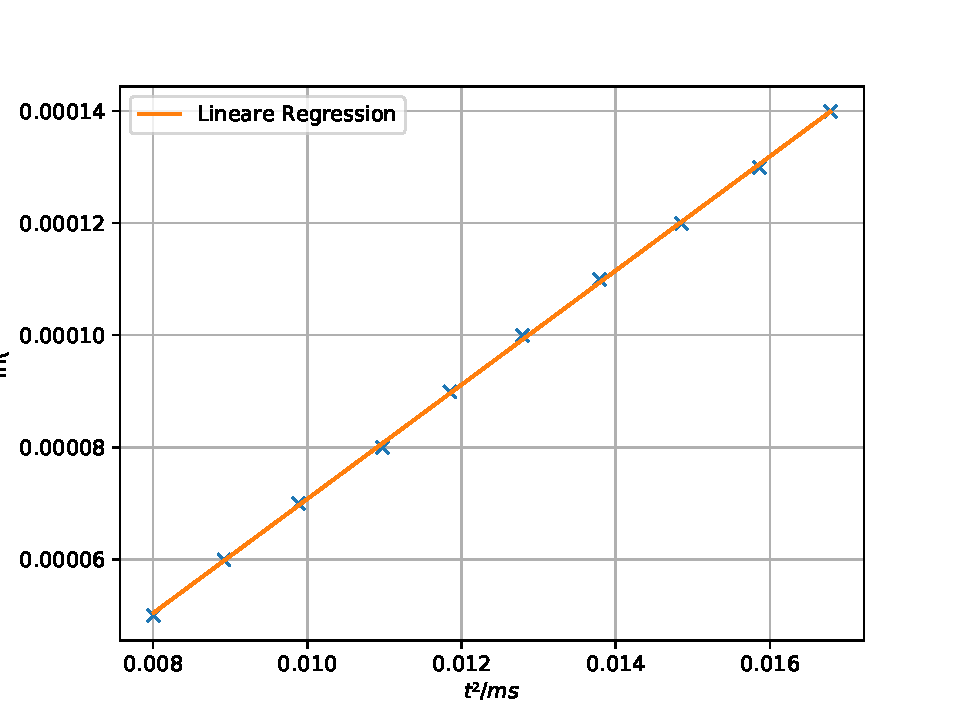
\includegraphics{Graphibitte.pdf}
%  \caption{Plot.}
%  \label{fig:plot}
%\end{figure}

%Einheiten: \SI{3}{\newton\s}
%1,41 \cdot \cramped{10^{-3}} ~s  für hochzahlen

%\begin{table}
%  \centering
%  \caption{Tabelle für a)Erste Bestimmung der Zeitkonstanten}
%  \label{Tab1}
%    \begin{tabular}{c c}%c zeigt die anzahl der Spalten
%      \toprule
%      Spannung $U_c$ &Zeit $t$\\% \\ werden benötigt um die Zeile zu Beenden
%      mV&ms\\% & Zeichen grenzen die Zahlen voneinander ab.
%      \midrule
%      \midrule
%        %\input{tab1.txt}% Die Tabelle ist hier ausgelagert. Sie kann aber auch genausogut hier eingefügt werden.
%          0,000 &     752\\
%          0,400 &     440\\
%          0,800 &     448\\
%      \bottomrule
%    \end{tabular}
%\end{table}

%\begin{table}
%    \centering
%    \caption{Messwerte für die Beta-Strahlung.}
%    \label{Tabg}
%    \sisetup{table-format=1.2}
%    \begin{tabular}{S S[table-format=2.2] S } %3 ziffern vom kommer, zwei danach, geht hiter jedes s
%      \toprule
%      %{$D$/cm}& \multicolumn{5}{c}{$U_{\symup{B}i} = \,\si{V}$}\\ überschrift über mehrere spalten
%      %\midrule
%       {$D/ \mu\si{m}$}& {$R/\frac{\si{kg}}{\si{m²}}$} & {$t$/s} &  {$N$} & {$A_{\symup{gem}} = \frac{N}{t}/ \frac{1}{\si{s}}$}  & {$A/ \frac{1}{\si{s}}$}  & {$\symup{ln}(A)$}\\
%      \midrule
%      \midrule
%          {$ 3924 \pm 62$} & 39,24 & {$ ~~3,652 \pm 0,016$}\\
%          {$ 2122 \pm 46$} & 10,61 & {$ ~~2,296 \pm 0,023$}\\
%          {$ 3001 \pm 54$} & 10,00 & {$ ~~2,233 \pm 0,019$}\\
%      \bottomrule
%    \end{tabular}
%\end{table}

%Mittelwert von X:
%\begin{equation*}
%  \overline{X }=  \frac{1}{N} \sum_{i=1}^N (X_i) = 75,98 \, \si{Hz} 
%\end{equation*}
%Formel für den Fehler des Mittelwerts:
%\begin{equation*}
%  \symup{\Delta} X = \frac{1}{\sqrt{N}} \sqrt{\frac{1}{\sqrt{N-1}} \sum_{i=1}^N (X_{i}-\overline{X})²}= 0,02 \, \si{Hz} 
%\end{equation*}

\subsection{Messung der Molwärme bei konstantem Druck und Berechnung der Molwärme bei konstantem Volumen}

Zunächst wurde der äußerer Probenzylinder der Apperatur, welche in der Durchführung beschrieben ist, mit 
flüssigem Stickstoff auf eine Temperatur von $T_0 = \SI{-189,5}{\celsius}$ gekühlt, da eine tiefere Temperatur 
nicht erreicht werden konnte. Von da an wurde die Heizspannung $U$, der Heizstrom $I$, der Widerstand $R$ 
und die Zeit $t$ die nötig ist um eine Temperaturerhöhung um etwa $10$ K zu erreichen, gemessen. Die Werte sind in Tabelle \ref{Tab1} 
dargestellt. Aus dem Widerstand in Ohm wurde mit der Formel 
\begin{equation*}
    T[\si{°C}] = 0,00134 \cdot (R[\symup{\Omega}])² + 2,296 \cdot R[\symup{\Omega}] -243,02
\end{equation*}
die Temperatur in Grad-Celsius berechnet und die entsprechnenden Werte für die Temperatur wurden 
in Tabelle \ref{Tab1} hinzugefügt. Außerdem wurde eine Umrechnung in Kelvin vorgenommen, 
wobei die Formel 
\begin{equation*}
    T[\si{K}] = T[\si{°C}] + 273,2
\end{equation*}
verwendet wurde. Die Näherung $273,15 \approx 273,2$ wurde verwendet, da die Temperatur mit der vorliegenden 
Messmethode nicht auf zwei Nachkommastellen genau bestimmt werden kann, und durch die Umrechnung in Kelvin 
keine solche Genauigkeit suggeriert werden sollte. 
Außerdem wurde in der Tabelle \ref{Tab1} die Temperaturdifferenz $\symup{\Delta}T$ angegeben, diese ergibt 
sich aus der Temperatur $T$ zum Messzeitpunkt der Zeit $t$, und der Temperatur davor. Für die erste 
Temperaturdifferenz wurden die Anfangstemperatur $T_0$ und $T=\SI{-180,1}{\celsius}$ verwendet, für die darauf 
immer die gemessene Endtemperatur und die Endtemperatur aus der vorherigen Messung.

\begin{table}
    \centering
    \caption{Messwerte für die Molwärmeberechnung und berechnete Werte einschließlich der Molwärme.}
    \label{Tab1}
    \sisetup{table-format=3.1}
    \begin{tabular}{S[table-format=2.1] S S S[table-format=2.1] S S S S S} %3 ziffern vom kommer, zwei danach, geht hiter jedes s
      \toprule
      %{$D$/cm}& \multicolumn{5}{c}{$U_{\symup{B}i} = \,\si{V}$}\\ überschrift über mehrere spalten
      %\midrule
       {$U/ \si{V}$}& {$I/\si{mA}$} & {$t$/s} & {$R/\symup{\Omega}$} & {$\symup{\Delta}T$/K} & {$T$/°C} & {$T$/K} & {$C_{\si{p}}$/$\frac{\si{J}}{\si{molK}}$} &{$C_{\si{v}}$/$\frac{\si{J}}{\si{molK}}$} \\
      \midrule
      \midrule
          {16,69} & {160,3}  & {$274$} & {~27,0} &  9,4 & {-180,1} &  93,1 & {14,5} & {14,4} \\
          {16,95} & {161,2}  & {$320$} & {~31,3} & 10,2 & {-169,8} & 103,4 & {15,9} & {15,8} \\
          {17,05} & {162,0}  & {$335$} & {~35,5} & 10,0 & {-159,8} & 113,4 & {17,1} & {17,1} \\
          {17,15} & {162,8}  & {$369$} & {~39,7} & 10,1 & {-149,8} & 123,4 & {19,0} & {18,9} \\
          {18,80} & {178,0}  & {$309$} & {~43,8} &  9,9 & {-139,9} & 133,3 & {19,5} & {19,3} \\
          {18,65} & {176,8}  & {$329$} & {~47,9} &  9,9 & {-130,2} & 143,0 & {20,3} & {20,1} \\
          {19,79} & {187,4}  & {$307$} & {~52,0} & 10,0 & {-120,0} & 153,2 & {21,2} & {21,0} \\
          {19,86} & {188,0}  & {$307$} & {~56,1} & 10,0 & {-110,0} & 163,2 & {21,3} & {21,0} \\
          {19,90} & {188,3}  & {$310$} & {~60,2} & 10,1 & {~-99,9} & 173,3 & {21,4} & {21,2} \\
          {19,93} & {188,5}  & {$317$} & {~64,3} & 10,1 & {~-89,8} & 183,4 & {21,9} & {21,6} \\
          {19,96} & {188,7}  & {$322$} & {~68,3} &  9,9 & {~-80,0} & 193,2 & {22,9} & {22,4} \\
          {19,98} & {188,9}  & {$326$} & {~72,3} &  9,9 & {~-70,0} & 203,2 & {23,0} & {22,6} \\
          {20,0 } & {189,1}  & {$324$} & {~76,3} & 10,0 & {~-60,0} & 213,2 & {22,9} & {22,4} \\
          {20,0 } & {189,2}  & {$300$} & {~80,3} & 10,0 & {~-50,0} & 223,2 & {21,0} & {20,6} \\
          {20,1 } & {189,3}  & {$379$} & {~84,2} &  9,8 & {~-40,2} & 233,0 & {27,3} & {26,8} \\
          {20,0 } & {189,4}  & {$367$} & {~88,2} & 10,1 & {~-30,2} & 243,0 & {25,6} & {25,1} \\
          {20,0 } & {189,5}  & {$266$} & {~92,1} &  9,9 & {~-20,2} & 253,0 & {19,0} & {18,4} \\
          {20,0 } & {189,5}  & {$367$} & {~96,1} & 10,2 & {~-10,0} & 263,2 & {25,4} & {24,8} \\
          {20,0 } & {189,6}  & {$371$} & {100,0} & 10,0 & {~~~0,0} & 273,2 & {26,2} & {25,6} \\
          {20,0 } & {189,6}  & {$383$} & {103,9} & 10,0 & {~~10,0} & 283,2 & {26,9} & {26,3} \\
          {20,0 } & {189,7}  & {$375$} & {107,8} & 10,1 & {~~20,1} & 293,3 & {26,3} & {25,6} \\
          {20,0 } & {189,8}  & {$375$} & {111,7} & 10,1 & {~~30,2} & 303,4 & {26,2} & {25,5} \\
      \bottomrule
    \end{tabular}
\end{table}
\FloatBarrier

Durch die Formel \ref{eqn:cp} wurde die Molwärme bei konstantem Druck $C_{\si{p}}$ berechnet, mit Formel 
\ref{eqn:cv} wird diese in Molwärme bei konstantem Volumen $C_{\si{v}}$ umgerechnet. Auch diese berechneten 
Werte sind in Tabelle \ref{Tab1} zu finden. Die Werte für den 
linaren Ausdehnungskoefizienten $\alpha$, die für die Berechnung der Molwärme bei konstantem Volumen notwendig 
sind, werden der Tabelle in Abbildung \ref{fig:a} entnommen. Dabei wird die 
Temperatur immer auf die nächste Zehnerpotenz abgerudet. Z.B. wird für den ersten Wert bei 
$T=\SI{93,1}{\kelvin}$ der lineare Ausdehnungskoefizient für den Wert von $\SI{90}{\kelvin}$ verwendet. 
Da die Molwärme bei konstantem Druck auf die erste Nachkommastelle gerundet wird, ist der entstehende 
Fehler vernachlässigbar.

Zur Veranschaulichung der Daten wird die Molwärme bei konstanten Volumen gegen die Temperatur aufgetragen. 
Der Graph ist in Abbildung \ref{fig:cv} zu sehen. 

\begin{figure}
  \centering
  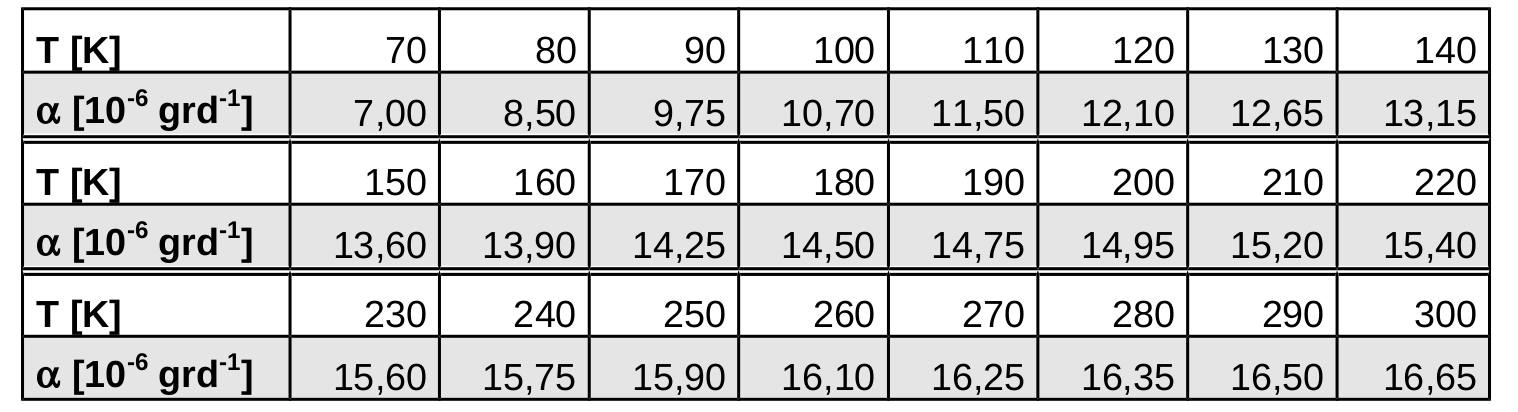
\includegraphics[width=0.95\textwidth]{alpha.png}
  \caption{Der lineare Ausdehnungskoefizient.}
  \label{fig:a}
\end{figure}

\begin{figure}
  \centering
  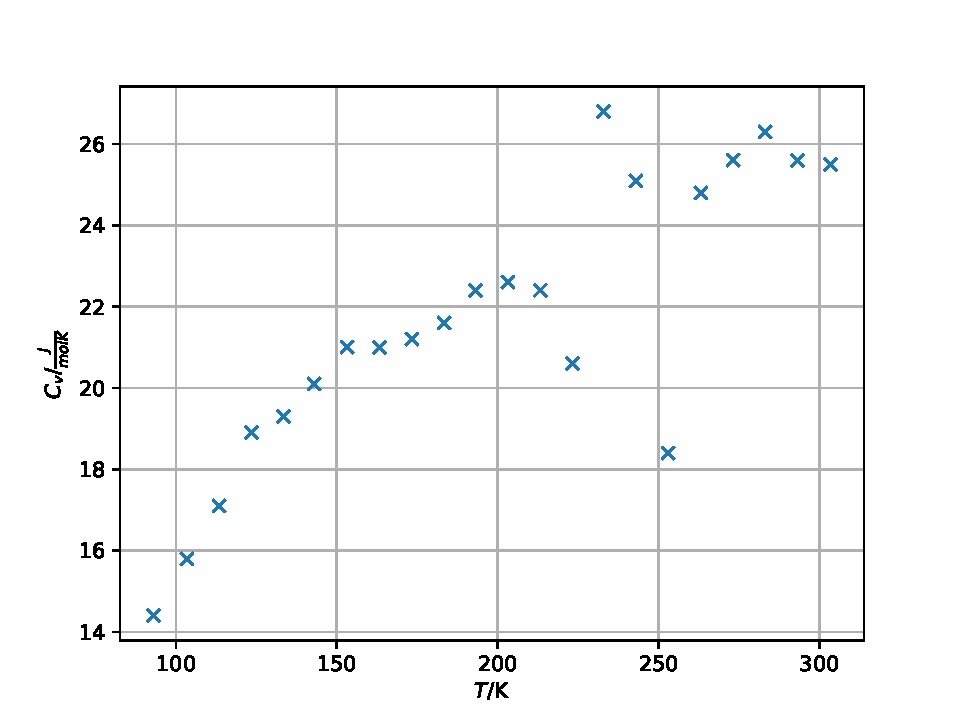
\includegraphics{cv.pdf}
  \caption{Die Molwärme bei konstantem Volumen in Abhängigkeit von der Temperatur.}
  \label{fig:cv}
\end{figure}






\subsection{Bestimmung der Debye-Temperatur}
 
 
 



 
 
 
 
 
 

 
 




